\documentclass[1p]{elsarticle_modified}
%\bibliographystyle{elsarticle-num}

%\usepackage[colorlinks]{hyperref}
%\usepackage{abbrmath_seonhwa} %\Abb, \Ascr, \Acal ,\Abf, \Afrak
\usepackage{amsfonts}
\usepackage{amssymb}
\usepackage{amsmath}
\usepackage{amsthm}
\usepackage{scalefnt}
\usepackage{amsbsy}
\usepackage{kotex}
\usepackage{caption}
\usepackage{subfig}
\usepackage{color}
\usepackage{graphicx}
\usepackage{xcolor} %% white, black, red, green, blue, cyan, magenta, yellow
\usepackage{float}
\usepackage{setspace}
\usepackage{hyperref}

\usepackage{tikz}
\usetikzlibrary{arrows}

\usepackage{multirow}
\usepackage{array} % fixed length table
\usepackage{hhline}

%%%%%%%%%%%%%%%%%%%%%
\makeatletter
\renewcommand*\env@matrix[1][\arraystretch]{%
	\edef\arraystretch{#1}%
	\hskip -\arraycolsep
	\let\@ifnextchar\new@ifnextchar
	\array{*\c@MaxMatrixCols c}}
\makeatother %https://tex.stackexchange.com/questions/14071/how-can-i-increase-the-line-spacing-in-a-matrix
%%%%%%%%%%%%%%%

\usepackage[normalem]{ulem}

\newcommand{\msout}[1]{\ifmmode\text{\sout{\ensuremath{#1}}}\else\sout{#1}\fi}
%SOURCE: \msout is \stkout macro in https://tex.stackexchange.com/questions/20609/strikeout-in-math-mode

\newcommand{\cancel}[1]{
	\ifmmode
	{\color{red}\msout{#1}}
	\else
	{\color{red}\sout{#1}}
	\fi
}

\newcommand{\add}[1]{
	{\color{blue}\uwave{#1}}
}

\newcommand{\replace}[2]{
	\ifmmode
	{\color{red}\msout{#1}}{\color{blue}\uwave{#2}}
	\else
	{\color{red}\sout{#1}}{\color{blue}\uwave{#2}}
	\fi
}

\newcommand{\Sol}{\mathcal{S}} %segment
\newcommand{\D}{D} %diagram
\newcommand{\A}{\mathcal{A}} %arc


%%%%%%%%%%%%%%%%%%%%%%%%%%%%%5 test

\def\sl{\operatorname{\textup{SL}}(2,\Cbb)}
\def\psl{\operatorname{\textup{PSL}}(2,\Cbb)}
\def\quan{\mkern 1mu \triangleright \mkern 1mu}

\theoremstyle{definition}
\newtheorem{thm}{Theorem}[section]
\newtheorem{prop}[thm]{Proposition}
\newtheorem{lem}[thm]{Lemma}
\newtheorem{ques}[thm]{Question}
\newtheorem{cor}[thm]{Corollary}
\newtheorem{defn}[thm]{Definition}
\newtheorem{exam}[thm]{Example}
\newtheorem{rmk}[thm]{Remark}
\newtheorem{alg}[thm]{Algorithm}

\newcommand{\I}{\sqrt{-1}}
\begin{document}

%\begin{frontmatter}
%
%\title{Boundary parabolic representations of knots up to 8 crossings}
%
%%% Group authors per affiliation:
%\author{Yunhi Cho} 
%\address{Department of Mathematics, University of Seoul, Seoul, Korea}
%\ead{yhcho@uos.ac.kr}
%
%
%\author{Seonhwa Kim} %\fnref{s_kim}}
%\address{Center for Geometry and Physics, Institute for Basic Science, Pohang, 37673, Korea}
%\ead{ryeona17@ibs.re.kr}
%
%\author{Hyuk Kim}
%\address{Department of Mathematical Sciences, Seoul National University, Seoul 08826, Korea}
%\ead{hyukkim@snu.ac.kr}
%
%\author{Seokbeom Yoon}
%\address{Department of Mathematical Sciences, Seoul National University, Seoul, 08826,  Korea}
%\ead{sbyoon15@snu.ac.kr}
%
%\begin{abstract}
%We find all boundary parabolic representation of knots up to 8 crossings.
%
%\end{abstract}
%\begin{keyword}
%    \MSC[2010] 57M25 
%\end{keyword}
%
%\end{frontmatter}

%\linenumbers
%\tableofcontents
%
\newcommand\colored[1]{\textcolor{white}{\rule[-0.35ex]{0.8em}{1.4ex}}\kern-0.8em\color{red} #1}%
%\newcommand\colored[1]{\textcolor{white}{ #1}\kern-2.17ex	\textcolor{white}{ #1}\kern-1.81ex	\textcolor{white}{ #1}\kern-2.15ex\color{red}#1	}

{\Large $\underline{12a_{0397}~(K12a_{0397})}$}

\setlength{\tabcolsep}{10pt}
\renewcommand{\arraystretch}{1.6}
\vspace{1cm}\begin{tabular}{m{100pt}>{\centering\arraybackslash}m{274pt}}
\multirow{5}{120pt}{
	\centering
	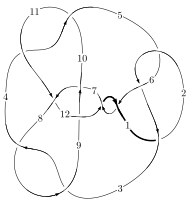
\includegraphics[width=112pt]{../../../GIT/diagram.site/Diagrams/png/1198_12a_0397.png}\\
\ \ \ A knot diagram\footnotemark}&
\allowdisplaybreaks
\textbf{Linearized knot diagam} \\
\cline{2-2}
 &
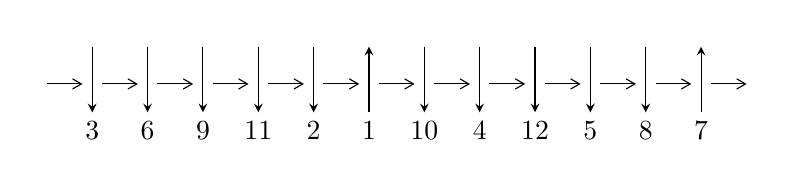
\begin{tikzpicture}[x=20pt, y=17pt]
	% nodes
	\node (C0) at (0, 0) {};
	\node (C1) at (1, 0) {};
	\node (C1U) at (1, +1) {};
	\node (C1D) at (1, -1) {3};

	\node (C2) at (2, 0) {};
	\node (C2U) at (2, +1) {};
	\node (C2D) at (2, -1) {6};

	\node (C3) at (3, 0) {};
	\node (C3U) at (3, +1) {};
	\node (C3D) at (3, -1) {9};

	\node (C4) at (4, 0) {};
	\node (C4U) at (4, +1) {};
	\node (C4D) at (4, -1) {11};

	\node (C5) at (5, 0) {};
	\node (C5U) at (5, +1) {};
	\node (C5D) at (5, -1) {2};

	\node (C6) at (6, 0) {};
	\node (C6U) at (6, +1) {};
	\node (C6D) at (6, -1) {1};

	\node (C7) at (7, 0) {};
	\node (C7U) at (7, +1) {};
	\node (C7D) at (7, -1) {10};

	\node (C8) at (8, 0) {};
	\node (C8U) at (8, +1) {};
	\node (C8D) at (8, -1) {4};

	\node (C9) at (9, 0) {};
	\node (C9U) at (9, +1) {};
	\node (C9D) at (9, -1) {12};

	\node (C10) at (10, 0) {};
	\node (C10U) at (10, +1) {};
	\node (C10D) at (10, -1) {5};

	\node (C11) at (11, 0) {};
	\node (C11U) at (11, +1) {};
	\node (C11D) at (11, -1) {8};

	\node (C12) at (12, 0) {};
	\node (C12U) at (12, +1) {};
	\node (C12D) at (12, -1) {7};
	\node (C13) at (13, 0) {};

	% arrows
	\draw[->,>={angle 60}]
	(C0) edge (C1) (C1) edge (C2) (C2) edge (C3) (C3) edge (C4) (C4) edge (C5) (C5) edge (C6) (C6) edge (C7) (C7) edge (C8) (C8) edge (C9) (C9) edge (C10) (C10) edge (C11) (C11) edge (C12) (C12) edge (C13) ;	\draw[->,>=stealth]
	(C1U) edge (C1D) (C2U) edge (C2D) (C3U) edge (C3D) (C4U) edge (C4D) (C5U) edge (C5D) (C6D) edge (C6U) (C7U) edge (C7D) (C8U) edge (C8D) (C9U) edge (C9D) (C10U) edge (C10D) (C11U) edge (C11D) (C12D) edge (C12U) ;
	\end{tikzpicture} \\
\hhline{~~} \\& 
\textbf{Solving Sequence} \\ \cline{2-2} 
 &
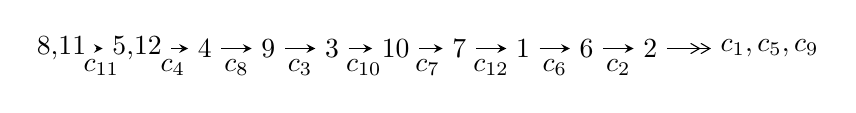
\begin{tikzpicture}[x=23pt, y=7pt]
	% node
	\node (A0) at (-1/8, 0) {8,11};
	\node (A1) at (17/16, 0) {5,12};
	\node (A2) at (17/8, 0) {4};
	\node (A3) at (25/8, 0) {9};
	\node (A4) at (33/8, 0) {3};
	\node (A5) at (41/8, 0) {10};
	\node (A6) at (49/8, 0) {7};
	\node (A7) at (57/8, 0) {1};
	\node (A8) at (65/8, 0) {6};
	\node (A9) at (73/8, 0) {2};
	\node (C1) at (1/2, -1) {$c_{11}$};
	\node (C2) at (13/8, -1) {$c_{4}$};
	\node (C3) at (21/8, -1) {$c_{8}$};
	\node (C4) at (29/8, -1) {$c_{3}$};
	\node (C5) at (37/8, -1) {$c_{10}$};
	\node (C6) at (45/8, -1) {$c_{7}$};
	\node (C7) at (53/8, -1) {$c_{12}$};
	\node (C8) at (61/8, -1) {$c_{6}$};
	\node (C9) at (69/8, -1) {$c_{2}$};
	\node (A10) at (11, 0) {$c_{1},c_{5},c_{9}$};

	% edge
	\draw[->,>=stealth]	
	(A0) edge (A1) (A1) edge (A2) (A2) edge (A3) (A3) edge (A4) (A4) edge (A5) (A5) edge (A6) (A6) edge (A7) (A7) edge (A8) (A8) edge (A9) ;
	\draw[->>,>={angle 60}]	
	(A9) edge (A10);
\end{tikzpicture} \\ 

\end{tabular} \\

\footnotetext{
The image of knot diagram is generated by the software ``\textbf{Draw programme}" developed by Andrew Bartholomew(\url{http://www.layer8.co.uk/maths/draw/index.htm\#Running-draw}), where we modified some parts for our purpose(\url{https://github.com/CATsTAILs/LinksPainter}).
}\phantom \\ \newline 
\centering \textbf{Ideals for irreducible components\footnotemark of $X_{\text{par}}$} 
 
\begin{align*}
I^u_{1}&=\langle 
1908269 u^{44}+69257295 u^{43}+\cdots+524288 b-1459838517248,\\
\phantom{I^u_{1}}&\phantom{= \langle  }-6600959 u^{44}-250923547 u^{43}+\cdots+1048576 a-5495160045568,\\
\phantom{I^u_{1}}&\phantom{= \langle  }u^{45}+39 u^{44}+\cdots+23068672 u+1048576\rangle \\
I^u_{2}&=\langle 
-4.69815\times10^{233} a^{39} u-6.24002\times10^{233} a^{38} u+\cdots-1.03893\times10^{237} a+1.05559\times10^{236},\\
\phantom{I^u_{2}}&\phantom{= \langle  }2 a^{39} u+21 a^{38} u+\cdots+142 a-33,\;u^2- u+1\rangle \\
I^u_{3}&=\langle 
-11 u^{22}-8 u^{21}+\cdots+b+40,\;-29 u^{22}-83 u^{21}+\cdots+a+3,\;u^{23}+2 u^{22}+\cdots- u+1\rangle \\
\\
\end{align*}
\raggedright * 3 irreducible components of $\dim_{\mathbb{C}}=0$, with total 148 representations.\\
\footnotetext{All coefficients of polynomials are rational numbers. But the coefficients are sometimes approximated in decimal forms when there is not enough margin.}
\newpage
\renewcommand{\arraystretch}{1}
\centering \section*{I. $I^u_{1}= \langle 1.91\times10^{6} u^{44}+6.93\times10^{7} u^{43}+\cdots+5.24\times10^{5} b-1.46\times10^{12},\;-6.60\times10^{6} u^{44}-2.51\times10^{8} u^{43}+\cdots+1.05\times10^{6} a-5.50\times10^{12},\;u^{45}+39 u^{44}+\cdots+23068672 u+1048576 \rangle$}
\flushleft \textbf{(i) Arc colorings}\\
\begin{tabular}{m{7pt} m{180pt} m{7pt} m{180pt} }
\flushright $a_{8}=$&$\begin{pmatrix}0\\u\end{pmatrix}$ \\
\flushright $a_{11}=$&$\begin{pmatrix}1\\0\end{pmatrix}$ \\
\flushright $a_{5}=$&$\begin{pmatrix}6.29517 u^{44}+239.299 u^{43}+\cdots+1.12427\times10^{8} u+5240593\\-3.63973 u^{44}-132.098 u^{43}+\cdots+5.32322\times10^{7} u+2784421\end{pmatrix}$ \\
\flushright $a_{12}=$&$\begin{pmatrix}1\\u^2\end{pmatrix}$ \\
\flushright $a_{4}=$&$\begin{pmatrix}2.65543 u^{44}+107.202 u^{43}+\cdots+1.65659\times10^{8} u+8025014\\-3.63973 u^{44}-132.098 u^{43}+\cdots+5.32322\times10^{7} u+2784421\end{pmatrix}$ \\
\flushright $a_{9}=$&$\begin{pmatrix}\frac{1}{1024} u^{43}+\frac{37}{1024} u^{42}+\cdots+10752 u+\frac{1025}{2}\\-0.000976563 u^{44}-0.0361328 u^{43}+\cdots-10752 u^{2}-511.500 u\end{pmatrix}$ \\
\flushright $a_{3}=$&$\begin{pmatrix}10.3764 u^{44}+403.507 u^{43}+\cdots+3.53442\times10^{8} u+1.68991\times10^{7}\\11.0232 u^{44}+424.937 u^{43}+\cdots+3.09218\times10^{8} u+1.46969\times10^{7}\end{pmatrix}$ \\
\flushright $a_{10}=$&$\begin{pmatrix}-0.000976563 u^{44}-0.0371094 u^{43}+\cdots-11264.5 u-511.500\\\frac{1}{1024} u^{44}+\frac{37}{1024} u^{43}+\cdots+10752 u^2+\frac{1025}{2} u\end{pmatrix}$ \\
\flushright $a_{7}=$&$\begin{pmatrix}\frac{1}{1024} u^{44}+\frac{45}{1024} u^{43}+\cdots+\frac{388097}{4} u+4608\\-\frac{7}{1024} u^{44}-\frac{17}{64} u^{43}+\cdots-154111 u-7168\end{pmatrix}$ \\
\flushright $a_{1}=$&$\begin{pmatrix}0.0998535 u^{44}+3.81567 u^{43}+\cdots+1630976 u+75265\\-0.0717773 u^{44}-2.68408 u^{43}+\cdots-383232 u-16128\end{pmatrix}$ \\
\flushright $a_{6}=$&$\begin{pmatrix}0.245605 u^{44}+8.91406 u^{43}+\cdots-2.76384\times10^{6} u-142464\\0.267578 u^{44}+10.4087 u^{43}+\cdots+7706241 u+364032\end{pmatrix}$ \\
\flushright $a_{2}=$&$\begin{pmatrix}-1.21094 u^{44}-46.2363 u^{43}+\cdots-2.15274\times10^{7} u-998527.\\-1.38721 u^{44}-52.9595 u^{43}+\cdots-2.50382\times10^{7} u-1163264\end{pmatrix}$\\&\end{tabular}
\flushleft \textbf{(ii) Obstruction class $= -1$}\\~\\
\flushleft \textbf{(iii) Cusp Shapes $= \frac{1487947}{65536} u^{44}+\frac{6940087}{8192} u^{43}+\cdots+108839472 u+4370874$}\\~\\
\newpage\renewcommand{\arraystretch}{1}
\flushleft \textbf{(iv) u-Polynomials at the component}\newline \\
\begin{tabular}{m{50pt}|m{274pt}}
Crossings & \hspace{64pt}u-Polynomials at each crossing \\
\hline $$\begin{aligned}c_{1}\end{aligned}$$&$\begin{aligned}
&u^{45}+24 u^{44}+\cdots+172 u+16
\end{aligned}$\\
\hline $$\begin{aligned}c_{2},c_{5}\end{aligned}$$&$\begin{aligned}
&u^{45}+6 u^{44}+\cdots+38 u+4
\end{aligned}$\\
\hline $$\begin{aligned}c_{3},c_{4},c_{8}\\c_{10}\end{aligned}$$&$\begin{aligned}
&u^{45}+15 u^{43}+\cdots+2 u+1
\end{aligned}$\\
\hline $$\begin{aligned}c_{6},c_{12}\end{aligned}$$&$\begin{aligned}
&u^{45}+18 u^{44}+\cdots+2834 u+188
\end{aligned}$\\
\hline $$\begin{aligned}c_{7},c_{9}\end{aligned}$$&$\begin{aligned}
&u^{45}+u^{44}+\cdots-7 u+1
\end{aligned}$\\
\hline $$\begin{aligned}c_{11}\end{aligned}$$&$\begin{aligned}
&u^{45}+39 u^{44}+\cdots+23068672 u+1048576
\end{aligned}$\\
\hline
\end{tabular}\\~\\
\newpage\renewcommand{\arraystretch}{1}
\flushleft \textbf{(v) Riley Polynomials at the component}\newline \\
\begin{tabular}{m{50pt}|m{274pt}}
Crossings & \hspace{64pt}Riley Polynomials at each crossing \\
\hline $$\begin{aligned}c_{1}\end{aligned}$$&$\begin{aligned}
&y^{45}-4 y^{44}+\cdots+11504 y-256
\end{aligned}$\\
\hline $$\begin{aligned}c_{2},c_{5}\end{aligned}$$&$\begin{aligned}
&y^{45}-24 y^{44}+\cdots+172 y-16
\end{aligned}$\\
\hline $$\begin{aligned}c_{3},c_{4},c_{8}\\c_{10}\end{aligned}$$&$\begin{aligned}
&y^{45}+30 y^{44}+\cdots+2 y-1
\end{aligned}$\\
\hline $$\begin{aligned}c_{6},c_{12}\end{aligned}$$&$\begin{aligned}
&y^{45}+32 y^{44}+\cdots+315660 y-35344
\end{aligned}$\\
\hline $$\begin{aligned}c_{7},c_{9}\end{aligned}$$&$\begin{aligned}
&y^{45}-21 y^{44}+\cdots+65 y-1
\end{aligned}$\\
\hline $$\begin{aligned}c_{11}\end{aligned}$$&$\begin{aligned}
&y^{45}-3 y^{44}+\cdots+9345848836096 y-1099511627776
\end{aligned}$\\
\hline
\end{tabular}\\~\\
\newpage\flushleft \textbf{(vi) Complex Volumes and Cusp Shapes}
$$\begin{array}{c|c|c}  
\text{Solutions to }I^u_{1}& \I (\text{vol} + \sqrt{-1}CS) & \text{Cusp shape}\\
 \hline 
\begin{aligned}
u &= -0.298816 + 0.989953 I \\
a &= -0.117552 - 1.073810 I \\
b &= -0.660784 + 0.641263 I\end{aligned}
 & -5.72982 - 2.27070 I & \phantom{-0.000000 } 0 \\ \hline\begin{aligned}
u &= -0.298816 - 0.989953 I \\
a &= -0.117552 + 1.073810 I \\
b &= -0.660784 - 0.641263 I\end{aligned}
 & -5.72982 + 2.27070 I & \phantom{-0.000000 } 0 \\ \hline\begin{aligned}
u &= -0.926262 + 0.495766 I \\
a &= \phantom{-}0.273491 - 0.286793 I \\
b &= -0.759181 - 0.337100 I\end{aligned}
 & -4.38180 + 2.50542 I & \phantom{-0.000000 } 0 \\ \hline\begin{aligned}
u &= -0.926262 - 0.495766 I \\
a &= \phantom{-}0.273491 + 0.286793 I \\
b &= -0.759181 + 0.337100 I\end{aligned}
 & -4.38180 - 2.50542 I & \phantom{-0.000000 } 0 \\ \hline\begin{aligned}
u &= -0.919385 + 0.529264 I \\
a &= -0.306815 + 0.321928 I \\
b &= \phantom{-}0.814984 + 0.335175 I\end{aligned}
 & -7.68302 + 7.12344 I & \phantom{-0.000000 } 0 \\ \hline\begin{aligned}
u &= -0.919385 - 0.529264 I \\
a &= -0.306815 - 0.321928 I \\
b &= \phantom{-}0.814984 - 0.335175 I\end{aligned}
 & -7.68302 - 7.12344 I & \phantom{-0.000000 } 0 \\ \hline\begin{aligned}
u &= -0.967769 + 0.504465 I \\
a &= -0.313757 + 0.244824 I \\
b &= \phantom{-}0.757522 + 0.405488 I\end{aligned}
 & -8.11430 - 1.70581 I & \phantom{-0.000000 } 0 \\ \hline\begin{aligned}
u &= -0.967769 - 0.504465 I \\
a &= -0.313757 - 0.244824 I \\
b &= \phantom{-}0.757522 - 0.405488 I\end{aligned}
 & -8.11430 + 1.70581 I & \phantom{-0.000000 } 0 \\ \hline\begin{aligned}
u &= -1.088800 + 0.239432 I \\
a &= \phantom{-}0.1243660 - 0.0152569 I \\
b &= -0.349735 - 0.420577 I\end{aligned}
 & -3.24070 - 0.55670 I & \phantom{-0.000000 } 0 \\ \hline\begin{aligned}
u &= -1.088800 - 0.239432 I \\
a &= \phantom{-}0.1243660 + 0.0152569 I \\
b &= -0.349735 + 0.420577 I\end{aligned}
 & -3.24070 + 0.55670 I & \phantom{-0.000000 } 0\\
 \hline 
 \end{array}$$\newpage$$\begin{array}{c|c|c}  
\text{Solutions to }I^u_{1}& \I (\text{vol} + \sqrt{-1}CS) & \text{Cusp shape}\\
 \hline 
\begin{aligned}
u &= -0.198202 + 1.097100 I \\
a &= \phantom{-}0.142561 + 1.104920 I \\
b &= \phantom{-}0.575831 - 0.709841 I\end{aligned}
 & -2.07839 + 2.22551 I & \phantom{-0.000000 } 0 \\ \hline\begin{aligned}
u &= -0.198202 - 1.097100 I \\
a &= \phantom{-}0.142561 - 1.104920 I \\
b &= \phantom{-}0.575831 + 0.709841 I\end{aligned}
 & -2.07839 - 2.22551 I & \phantom{-0.000000 } 0 \\ \hline\begin{aligned}
u &= -0.748453 + 0.420636 I \\
a &= \phantom{-}0.044813 - 0.385321 I \\
b &= -0.672626 - 0.096659 I\end{aligned}
 & -1.42425 + 3.31805 I & \phantom{-0.000000 } 0 \\ \hline\begin{aligned}
u &= -0.748453 - 0.420636 I \\
a &= \phantom{-}0.044813 + 0.385321 I \\
b &= -0.672626 + 0.096659 I\end{aligned}
 & -1.42425 - 3.31805 I & \phantom{-0.000000 } 0 \\ \hline\begin{aligned}
u &= \phantom{-}1.137450 + 0.415999 I \\
a &= \phantom{-}0.056535 + 1.223700 I \\
b &= \phantom{-}0.076306 - 0.677052 I\end{aligned}
 & \phantom{-}1.92192 + 2.39939 I & \phantom{-0.000000 } 0 \\ \hline\begin{aligned}
u &= \phantom{-}1.137450 - 0.415999 I \\
a &= \phantom{-}0.056535 - 1.223700 I \\
b &= \phantom{-}0.076306 + 0.677052 I\end{aligned}
 & \phantom{-}1.92192 - 2.39939 I & \phantom{-0.000000 } 0 \\ \hline\begin{aligned}
u &= -0.316288 + 1.178330 I \\
a &= -0.124276 - 1.126580 I \\
b &= -0.636773 + 0.790453 I\end{aligned}
 & -5.70018 + 6.82908 I & \phantom{-0.000000 } 0 \\ \hline\begin{aligned}
u &= -0.316288 - 1.178330 I \\
a &= -0.124276 + 1.126580 I \\
b &= -0.636773 - 0.790453 I\end{aligned}
 & -5.70018 - 6.82908 I & \phantom{-0.000000 } 0 \\ \hline\begin{aligned}
u &= -0.489115 + 0.309548 I \\
a &= \phantom{-}0.313689 + 0.454525 I \\
b &= \phantom{-}0.529742 - 0.075882 I\end{aligned}
 & -0.730208 - 0.083656 I & \phantom{-0.000000 } 0 \\ \hline\begin{aligned}
u &= -0.489115 - 0.309548 I \\
a &= \phantom{-}0.313689 - 0.454525 I \\
b &= \phantom{-}0.529742 + 0.075882 I\end{aligned}
 & -0.730208 + 0.083656 I & \phantom{-0.000000 } 0\\
 \hline 
 \end{array}$$\newpage$$\begin{array}{c|c|c}  
\text{Solutions to }I^u_{1}& \I (\text{vol} + \sqrt{-1}CS) & \text{Cusp shape}\\
 \hline 
\begin{aligned}
u &= -0.497869\phantom{ +0.000000I} \\
a &= \phantom{-}0.450653\phantom{ +0.000000I} \\
b &= \phantom{-}0.446828\phantom{ +0.000000I}\end{aligned}
 & -0.768321\phantom{ +0.000000I} & \phantom{-0.000000 } 0 \\ \hline\begin{aligned}
u &= -0.87680 + 1.39604 I \\
a &= -0.302809 - 1.259470 I \\
b &= -0.61138 + 1.39569 I\end{aligned}
 & -1.64377 + 9.31582 I & \phantom{-0.000000 } 0 \\ \hline\begin{aligned}
u &= -0.87680 - 1.39604 I \\
a &= -0.302809 + 1.259470 I \\
b &= -0.61138 - 1.39569 I\end{aligned}
 & -1.64377 - 9.31582 I & \phantom{-0.000000 } 0 \\ \hline\begin{aligned}
u &= -0.90557 + 1.38569 I \\
a &= -0.325344 - 1.265460 I \\
b &= -0.59960 + 1.43721 I\end{aligned}
 & -0.4610 + 18.4165 I & \phantom{-0.000000 } 0 \\ \hline\begin{aligned}
u &= -0.90557 - 1.38569 I \\
a &= -0.325344 + 1.265460 I \\
b &= -0.59960 - 1.43721 I\end{aligned}
 & -0.4610 - 18.4165 I & \phantom{-0.000000 } 0 \\ \hline\begin{aligned}
u &= -0.89990 + 1.39988 I \\
a &= \phantom{-}0.319514 + 1.255210 I \\
b &= \phantom{-}0.58882 - 1.41851 I\end{aligned}
 & \phantom{-}2.67201 + 13.38930 I & \phantom{-0.000000 } 0 \\ \hline\begin{aligned}
u &= -0.89990 - 1.39988 I \\
a &= \phantom{-}0.319514 - 1.255210 I \\
b &= \phantom{-}0.58882 + 1.41851 I\end{aligned}
 & \phantom{-}2.67201 - 13.38930 I & \phantom{-0.000000 } 0 \\ \hline\begin{aligned}
u &= -1.66275 + 0.46895 I \\
a &= -0.248878 - 0.405451 I \\
b &= \phantom{-}0.210659 + 0.990181 I\end{aligned}
 & -4.73342 - 0.73218 I & \phantom{-0.000000 } 0 \\ \hline\begin{aligned}
u &= -1.66275 - 0.46895 I \\
a &= -0.248878 + 0.405451 I \\
b &= \phantom{-}0.210659 - 0.990181 I\end{aligned}
 & -4.73342 + 0.73218 I & \phantom{-0.000000 } 0 \\ \hline\begin{aligned}
u &= -0.77091 + 1.54748 I \\
a &= \phantom{-}0.250065 + 1.181600 I \\
b &= \phantom{-}0.520537 - 1.229120 I\end{aligned}
 & \phantom{-}1.55549 + 7.27021 I & \phantom{-0.000000 } 0\\
 \hline 
 \end{array}$$\newpage$$\begin{array}{c|c|c}  
\text{Solutions to }I^u_{1}& \I (\text{vol} + \sqrt{-1}CS) & \text{Cusp shape}\\
 \hline 
\begin{aligned}
u &= -0.77091 - 1.54748 I \\
a &= \phantom{-}0.250065 - 1.181600 I \\
b &= \phantom{-}0.520537 + 1.229120 I\end{aligned}
 & \phantom{-}1.55549 - 7.27021 I & \phantom{-0.000000 } 0 \\ \hline\begin{aligned}
u &= -0.93055 + 1.47612 I \\
a &= \phantom{-}0.326629 + 1.202060 I \\
b &= \phantom{-}0.49630 - 1.38462 I\end{aligned}
 & \phantom{-}6.74317 + 12.42830 I & \phantom{-0.000000 } 0 \\ \hline\begin{aligned}
u &= -0.93055 - 1.47612 I \\
a &= \phantom{-}0.326629 - 1.202060 I \\
b &= \phantom{-}0.49630 + 1.38462 I\end{aligned}
 & \phantom{-}6.74317 - 12.42830 I & \phantom{-0.000000 } 0 \\ \hline\begin{aligned}
u &= -0.92821 + 1.52975 I \\
a &= -0.314902 - 1.176640 I \\
b &= -0.46221 + 1.34602 I\end{aligned}
 & \phantom{-}7.57419 + 7.55749 I & \phantom{-0.000000 } 0 \\ \hline\begin{aligned}
u &= -0.92821 - 1.52975 I \\
a &= -0.314902 + 1.176640 I \\
b &= -0.46221 - 1.34602 I\end{aligned}
 & \phantom{-}7.57419 - 7.55749 I & \phantom{-0.000000 } 0 \\ \hline\begin{aligned}
u &= -1.75215 + 0.63639 I \\
a &= -0.297374 - 0.502556 I \\
b &= \phantom{-}0.198323 + 1.086910 I\end{aligned}
 & -3.21485 - 9.54783 I & \phantom{-0.000000 } 0 \\ \hline\begin{aligned}
u &= -1.75215 - 0.63639 I \\
a &= -0.297374 + 0.502556 I \\
b &= \phantom{-}0.198323 - 1.086910 I\end{aligned}
 & -3.21485 + 9.54783 I & \phantom{-0.000000 } 0 \\ \hline\begin{aligned}
u &= -1.80049 + 0.55270 I \\
a &= \phantom{-}0.247640 + 0.493732 I \\
b &= -0.168749 - 1.056050 I\end{aligned}
 & -0.29405 - 4.47039 I & \phantom{-0.000000 } 0 \\ \hline\begin{aligned}
u &= -1.80049 - 0.55270 I \\
a &= \phantom{-}0.247640 - 0.493732 I \\
b &= -0.168749 + 1.056050 I\end{aligned}
 & -0.29405 + 4.47039 I & \phantom{-0.000000 } 0 \\ \hline\begin{aligned}
u &= -0.87811 + 1.69637 I \\
a &= -0.272990 - 1.129230 I \\
b &= -0.400769 + 1.241740 I\end{aligned}
 & \phantom{-}6.69869 + 5.23471 I & \phantom{-0.000000 } 0\\
 \hline 
 \end{array}$$\newpage$$\begin{array}{c|c|c}  
\text{Solutions to }I^u_{1}& \I (\text{vol} + \sqrt{-1}CS) & \text{Cusp shape}\\
 \hline 
\begin{aligned}
u &= -0.87811 - 1.69637 I \\
a &= -0.272990 + 1.129230 I \\
b &= -0.400769 - 1.241740 I\end{aligned}
 & \phantom{-}6.69869 - 5.23471 I & \phantom{-0.000000 } 0 \\ \hline\begin{aligned}
u &= -0.84113 + 1.84473 I \\
a &= \phantom{-}0.248866 + 1.102950 I \\
b &= \phantom{-}0.356157 - 1.185750 I\end{aligned}
 & \phantom{-}4.90627 + 0.20772 I & \phantom{-0.000000 } 0 \\ \hline\begin{aligned}
u &= -0.84113 - 1.84473 I \\
a &= \phantom{-}0.248866 - 1.102950 I \\
b &= \phantom{-}0.356157 + 1.185750 I\end{aligned}
 & \phantom{-}4.90627 - 0.20772 I & \phantom{-0.000000 } 0 \\ \hline\begin{aligned}
u &= -2.18886 + 0.16892 I \\
a &= \phantom{-}0.051200 + 0.568765 I \\
b &= -0.026784 - 1.043710 I\end{aligned}
 & \phantom{-}2.93772 - 2.57806 I & \phantom{-0.000000 } 0 \\ \hline\begin{aligned}
u &= -2.18886 - 0.16892 I \\
a &= \phantom{-}0.051200 - 0.568765 I \\
b &= -0.026784 + 1.043710 I\end{aligned}
 & \phantom{-}2.93772 + 2.57806 I & \phantom{-0.000000 } 0\\
 \hline 
 \end{array}$$\newpage\newpage\renewcommand{\arraystretch}{1}
\centering \section*{II. $I^u_{2}= \langle -4.70\times10^{233} a^{39} u-6.24\times10^{233} a^{38} u+\cdots-1.04\times10^{237} a+1.06\times10^{236},\;2 a^{39} u+21 a^{38} u+\cdots+142 a-33,\;u^2- u+1 \rangle$}
\flushleft \textbf{(i) Arc colorings}\\
\begin{tabular}{m{7pt} m{180pt} m{7pt} m{180pt} }
\flushright $a_{8}=$&$\begin{pmatrix}0\\u\end{pmatrix}$ \\
\flushright $a_{11}=$&$\begin{pmatrix}1\\0\end{pmatrix}$ \\
\flushright $a_{5}=$&$\begin{pmatrix}a\\0.00205561 a^{39} u+0.00273024 a^{38} u+\cdots+4.54569 a-0.461858\end{pmatrix}$ \\
\flushright $a_{12}=$&$\begin{pmatrix}1\\u-1\end{pmatrix}$ \\
\flushright $a_{4}=$&$\begin{pmatrix}0.00205561 a^{39} u+0.00273024 a^{38} u+\cdots+5.54569 a-0.461858\\0.00205561 a^{39} u+0.00273024 a^{38} u+\cdots+4.54569 a-0.461858\end{pmatrix}$ \\
\flushright $a_{9}=$&$\begin{pmatrix}-0.000862208 a^{39} u+0.000899759 a^{38} u+\cdots-0.242076 a+0.813630\\-0.000364350 a^{39} u+0.00216092 a^{38} u+\cdots+0.166117 a+0.454919\end{pmatrix}$ \\
\flushright $a_{3}=$&$\begin{pmatrix}-0.000192689 a^{39} u-0.00330351 a^{38} u+\cdots+4.35116 a+0.103482\\-0.00192222 a^{39} u+0.000432146 a^{38} u+\cdots+1.19703 a-0.0456529\end{pmatrix}$ \\
\flushright $a_{10}=$&$\begin{pmatrix}0.000862208 a^{39} u-0.000899759 a^{38} u+\cdots+0.242076 a+1.18637\\-0.00308448 a^{39} u+0.00143811 a^{38} u+\cdots-1.13442 a-1.20040\end{pmatrix}$ \\
\flushright $a_{7}=$&$\begin{pmatrix}0.000354572 a^{39} u-0.000538750 a^{38} u+\cdots-0.171861 a+0.357600\\0.000286009 a^{39} u+0.000105031 a^{38} u+\cdots+0.617988 a+0.351373\end{pmatrix}$ \\
\flushright $a_{1}=$&$\begin{pmatrix}-0.0000706296 a^{39} u-0.000562200 a^{38} u+\cdots+0.412914 a-0.859285\\0.00181884 a^{39} u+0.00345821 a^{38} u+\cdots-0.844918 a-0.506231\end{pmatrix}$ \\
\flushright $a_{6}=$&$\begin{pmatrix}-0.00463429 a^{39} u-0.00244524 a^{38} u+\cdots+1.18427 a+2.37145\\0.00370820 a^{39} u+0.00576929 a^{38} u+\cdots-1.20106 a-2.81103\end{pmatrix}$ \\
\flushright $a_{2}=$&$\begin{pmatrix}-0.00374070 a^{39} u+0.00316369 a^{38} u+\cdots-8.66531 a-1.32879\\-0.00721432 a^{39} u+0.00732931 a^{38} u+\cdots-5.27593 a+1.01325\end{pmatrix}$\\&\end{tabular}
\flushleft \textbf{(ii) Obstruction class $= -1$}\\~\\
\flushleft \textbf{(iii) Cusp Shapes $= 0.0241933 a^{39} u+0.0327742 a^{38} u+\cdots+13.1336 a-21.3800$}\\~\\
\newpage\renewcommand{\arraystretch}{1}
\flushleft \textbf{(iv) u-Polynomials at the component}\newline \\
\begin{tabular}{m{50pt}|m{274pt}}
Crossings & \hspace{64pt}u-Polynomials at each crossing \\
\hline $$\begin{aligned}c_{1}\end{aligned}$$&$\begin{aligned}
&(u^{20}+11 u^{19}+\cdots+2 u+1)^{4}
\end{aligned}$\\
\hline $$\begin{aligned}c_{2},c_{5}\end{aligned}$$&$\begin{aligned}
&(u^{20}- u^{19}+\cdots+2 u-1)^{4}
\end{aligned}$\\
\hline $$\begin{aligned}c_{3},c_{4},c_{8}\\c_{10}\end{aligned}$$&$\begin{aligned}
&u^{80}- u^{79}+\cdots+35792 u+15097
\end{aligned}$\\
\hline $$\begin{aligned}c_{6},c_{12}\end{aligned}$$&$\begin{aligned}
&(u^{20}-3 u^{19}+\cdots-12 u+1)^{4}
\end{aligned}$\\
\hline $$\begin{aligned}c_{7},c_{9}\end{aligned}$$&$\begin{aligned}
&u^{80}-21 u^{79}+\cdots+36 u+169
\end{aligned}$\\
\hline $$\begin{aligned}c_{11}\end{aligned}$$&$\begin{aligned}
&(u^2- u+1)^{40}
\end{aligned}$\\
\hline
\end{tabular}\\~\\
\newpage\renewcommand{\arraystretch}{1}
\flushleft \textbf{(v) Riley Polynomials at the component}\newline \\
\begin{tabular}{m{50pt}|m{274pt}}
Crossings & \hspace{64pt}Riley Polynomials at each crossing \\
\hline $$\begin{aligned}c_{1}\end{aligned}$$&$\begin{aligned}
&(y^{20}-3 y^{19}+\cdots-6 y+1)^{4}
\end{aligned}$\\
\hline $$\begin{aligned}c_{2},c_{5}\end{aligned}$$&$\begin{aligned}
&(y^{20}-11 y^{19}+\cdots-2 y+1)^{4}
\end{aligned}$\\
\hline $$\begin{aligned}c_{3},c_{4},c_{8}\\c_{10}\end{aligned}$$&$\begin{aligned}
&y^{80}+63 y^{79}+\cdots+4240509516 y+227919409
\end{aligned}$\\
\hline $$\begin{aligned}c_{6},c_{12}\end{aligned}$$&$\begin{aligned}
&(y^{20}+17 y^{19}+\cdots-62 y+1)^{4}
\end{aligned}$\\
\hline $$\begin{aligned}c_{7},c_{9}\end{aligned}$$&$\begin{aligned}
&y^{80}+11 y^{79}+\cdots-716504 y+28561
\end{aligned}$\\
\hline $$\begin{aligned}c_{11}\end{aligned}$$&$\begin{aligned}
&(y^2+y+1)^{40}
\end{aligned}$\\
\hline
\end{tabular}\\~\\
\newpage\flushleft \textbf{(vi) Complex Volumes and Cusp Shapes}
$$\begin{array}{c|c|c}  
\text{Solutions to }I^u_{2}& \I (\text{vol} + \sqrt{-1}CS) & \text{Cusp shape}\\
 \hline 
\begin{aligned}
u &= \phantom{-}0.500000 + 0.866025 I \\
a &= \phantom{-}0.223301 - 0.984504 I \\
b &= -0.721069 + 0.935523 I\end{aligned}
 & -5.08534 + 7.61442 I & -9.65468 - 2.74133 I \\ \hline\begin{aligned}
u &= \phantom{-}0.500000 + 0.866025 I \\
a &= -0.161727 + 0.977147 I \\
b &= \phantom{-}0.679884 - 0.852689 I\end{aligned}
 & -1.84893 + 2.76931 I & -6.69810 + 0.36946 I \\ \hline\begin{aligned}
u &= \phantom{-}0.500000 + 0.866025 I \\
a &= -0.872992 + 0.525012 I \\
b &= -0.450422 - 1.018540 I\end{aligned}
 & \phantom{-}3.95796 - 2.02988 I & -8.93879 + 3.46410 I \\ \hline\begin{aligned}
u &= \phantom{-}0.500000 + 0.866025 I \\
a &= \phantom{-}0.521612 + 0.826124 I \\
b &= \phantom{-}0.311528 - 0.160068 I\end{aligned}
 & \phantom{-}1.94981 + 2.81121 I & -5.63163 - 2.91571 I \\ \hline\begin{aligned}
u &= \phantom{-}0.500000 + 0.866025 I \\
a &= -0.499155 + 0.940951 I \\
b &= -0.65006 - 1.49725 I\end{aligned}
 & \phantom{-}6.19099 - 3.97633 I & \phantom{-}0.94680 + 8.28286 I \\ \hline\begin{aligned}
u &= \phantom{-}0.500000 + 0.866025 I \\
a &= \phantom{-}0.171118 - 0.891526 I \\
b &= -0.788373 + 0.790387 I\end{aligned}
 & -5.88315 - 1.39328 I & -10.96035 + 3.63399 I \\ \hline\begin{aligned}
u &= \phantom{-}0.500000 + 0.866025 I \\
a &= -0.417061 + 0.760824 I \\
b &= -0.83097 - 1.32637 I\end{aligned}
 & \phantom{-}4.01885 - 3.83436 I & -2.82463 + 7.16468 I \\ \hline\begin{aligned}
u &= \phantom{-}0.500000 + 0.866025 I \\
a &= \phantom{-}0.355095 - 0.780475 I \\
b &= \phantom{-}0.90175 + 1.37031 I\end{aligned}
 & \phantom{-}0.92426 - 8.30305 I & -6.10015 + 10.00758 I \\ \hline\begin{aligned}
u &= \phantom{-}0.500000 + 0.866025 I \\
a &= \phantom{-}0.531113 - 1.032670 I \\
b &= \phantom{-}0.54401 + 1.57078 I\end{aligned}
 & \phantom{-}6.19099 - 0.08344 I & \phantom{-}0.94680 - 1.35465 I \\ \hline\begin{aligned}
u &= \phantom{-}0.500000 + 0.866025 I \\
a &= \phantom{-}0.375110 - 0.675074 I \\
b &= \phantom{-}0.90343 + 1.23362 I\end{aligned}
 & \phantom{-}0.496471 + 0.114015 I & -7.45592 + 3.22103 I\\
 \hline 
 \end{array}$$\newpage$$\begin{array}{c|c|c}  
\text{Solutions to }I^u_{2}& \I (\text{vol} + \sqrt{-1}CS) & \text{Cusp shape}\\
 \hline 
\begin{aligned}
u &= \phantom{-}0.500000 + 0.866025 I \\
a &= -0.528289 + 1.180870 I \\
b &= -0.35513 - 1.72050 I\end{aligned}
 & \phantom{-}0.92426 + 4.24328 I & -8.00000 + 0. I\phantom{ +0.000000I} \\ \hline\begin{aligned}
u &= \phantom{-}0.500000 + 0.866025 I \\
a &= \phantom{-}0.560866 - 1.168870 I \\
b &= \phantom{-}0.35123 + 1.65493 I\end{aligned}
 & \phantom{-}4.01885 - 0.22541 I & \phantom{-0.000000 } 0 \\ \hline\begin{aligned}
u &= \phantom{-}0.500000 + 0.866025 I \\
a &= -0.455734 - 0.521331 I \\
b &= -0.539610 - 0.030941 I\end{aligned}
 & \phantom{-}2.99206 - 1.44519 I & -3.20205 + 3.45501 I \\ \hline\begin{aligned}
u &= \phantom{-}0.500000 + 0.866025 I \\
a &= -0.565033 + 1.216060 I \\
b &= -0.26427 - 1.66859 I\end{aligned}
 & \phantom{-}0.49647 - 4.17378 I & \phantom{-0.000000 } 0 \\ \hline\begin{aligned}
u &= \phantom{-}0.500000 + 0.866025 I \\
a &= -0.17739 + 1.40437 I \\
b &= \phantom{-}0.160251 - 1.054550 I\end{aligned}
 & \phantom{-}1.94981 + 2.81121 I & \phantom{-0.000000 } 0 \\ \hline\begin{aligned}
u &= \phantom{-}0.500000 + 0.866025 I \\
a &= \phantom{-}0.043628 + 0.507114 I \\
b &= \phantom{-}0.928213 - 0.215774 I\end{aligned}
 & -1.59840 - 2.02988 I & -11.89977 + 3.46410 I \\ \hline\begin{aligned}
u &= \phantom{-}0.500000 + 0.866025 I \\
a &= \phantom{-}0.87299 - 1.27368 I \\
b &= \phantom{-}0.234300 + 1.392880 I\end{aligned}
 & \phantom{-}3.95796 - 2.02988 I & \phantom{-0.000000 } 0 \\ \hline\begin{aligned}
u &= \phantom{-}0.500000 + 0.866025 I \\
a &= \phantom{-}1.55443 - 0.33903 I \\
b &= \phantom{-}0.022743 + 0.944463 I\end{aligned}
 & \phantom{-}0.49647 - 4.17378 I & \phantom{-0.000000 } 0 \\ \hline\begin{aligned}
u &= \phantom{-}0.500000 + 0.866025 I \\
a &= \phantom{-}0.27721 - 1.58998 I \\
b &= \phantom{-}0.019390 + 1.138130 I\end{aligned}
 & \phantom{-}2.99206 - 1.44519 I & \phantom{-0.000000 } 0 \\ \hline\begin{aligned}
u &= \phantom{-}0.500000 + 0.866025 I \\
a &= \phantom{-}0.54980 + 1.52611 I \\
b &= -0.151295 - 0.510966 I\end{aligned}
 & -1.84893 + 2.76931 I & \phantom{-0.000000 } 0\\
 \hline 
 \end{array}$$\newpage$$\begin{array}{c|c|c}  
\text{Solutions to }I^u_{2}& \I (\text{vol} + \sqrt{-1}CS) & \text{Cusp shape}\\
 \hline 
\begin{aligned}
u &= \phantom{-}0.500000 + 0.866025 I \\
a &= -1.57372 + 0.50963 I \\
b &= -0.035102 - 1.032930 I\end{aligned}
 & \phantom{-}4.01885 - 0.22541 I & \phantom{-0.000000 } 0 \\ \hline\begin{aligned}
u &= \phantom{-}0.500000 + 0.866025 I \\
a &= -0.223415 - 0.228493 I \\
b &= -0.909375 - 0.182307 I\end{aligned}
 & \phantom{-}2.99206 - 2.61458 I & -3.20205 + 3.47320 I \\ \hline\begin{aligned}
u &= \phantom{-}0.500000 + 0.866025 I \\
a &= -0.65612 - 1.54780 I \\
b &= \phantom{-}0.206465 + 0.455571 I\end{aligned}
 & -5.08534 + 7.61442 I & \phantom{-0.000000 } 0 \\ \hline\begin{aligned}
u &= \phantom{-}0.500000 + 0.866025 I \\
a &= \phantom{-}0.157128 - 0.259381 I \\
b &= -1.328830 + 0.069336 I\end{aligned}
 & -5.88315 - 2.66649 I & -10.96035 + 3.29421 I \\ \hline\begin{aligned}
u &= \phantom{-}0.500000 + 0.866025 I \\
a &= -0.51135 - 1.66307 I \\
b &= \phantom{-}0.221039 + 0.585128 I\end{aligned}
 & -5.88315 - 1.39328 I & \phantom{-0.000000 } 0 \\ \hline\begin{aligned}
u &= \phantom{-}0.500000 + 0.866025 I \\
a &= -0.132043 + 0.215117 I \\
b &= \phantom{-}1.324980 + 0.002145 I\end{aligned}
 & -1.84893 - 6.82908 I & -6.69810 + 6.55874 I \\ \hline\begin{aligned}
u &= \phantom{-}0.500000 + 0.866025 I \\
a &= \phantom{-}0.161659 - 0.191649 I \\
b &= -1.376880 - 0.014061 I\end{aligned}
 & -5.08534 - 11.67420 I & -9.65468 + 9.66953 I \\ \hline\begin{aligned}
u &= \phantom{-}0.500000 + 0.866025 I \\
a &= \phantom{-}1.69318 - 0.48218 I \\
b &= -0.025625 + 1.034880 I\end{aligned}
 & \phantom{-}0.92426 + 4.24328 I & \phantom{-0.000000 } 0 \\ \hline\begin{aligned}
u &= \phantom{-}0.500000 + 0.866025 I \\
a &= -1.56080 + 0.88587 I \\
b &= -0.071541 - 1.200140 I\end{aligned}
 & \phantom{-}6.19099 - 0.08344 I & \phantom{-0.000000 } 0 \\ \hline\begin{aligned}
u &= \phantom{-}0.500000 + 0.866025 I \\
a &= \phantom{-}0.068505 + 0.163465 I \\
b &= \phantom{-}1.111960 + 0.176330 I\end{aligned}
 & \phantom{-}1.94981 - 6.87098 I & -5.63163 + 9.84391 I\\
 \hline 
 \end{array}$$\newpage$$\begin{array}{c|c|c}  
\text{Solutions to }I^u_{2}& \I (\text{vol} + \sqrt{-1}CS) & \text{Cusp shape}\\
 \hline 
\begin{aligned}
u &= \phantom{-}0.500000 + 0.866025 I \\
a &= \phantom{-}1.52884 - 1.08774 I \\
b &= \phantom{-}0.092842 + 1.273400 I\end{aligned}
 & \phantom{-}6.19099 - 3.97633 I & \phantom{-0.000000 } 0 \\ \hline\begin{aligned}
u &= \phantom{-}0.500000 + 0.866025 I \\
a &= -0.04363 + 1.89905 I \\
b &= -0.233613 - 0.987309 I\end{aligned}
 & -1.59840 - 2.02988 I & \phantom{-0.000000 } 0 \\ \hline\begin{aligned}
u &= \phantom{-}0.500000 + 0.866025 I \\
a &= \phantom{-}0.40194 - 1.88281 I \\
b &= \phantom{-}0.210631 + 1.186430 I\end{aligned}
 & \phantom{-}2.99206 - 2.61458 I & \phantom{-0.000000 } 0 \\ \hline\begin{aligned}
u &= \phantom{-}0.500000 + 0.866025 I \\
a &= \phantom{-}1.42992 - 1.42006 I \\
b &= \phantom{-}0.134239 + 1.363600 I\end{aligned}
 & \phantom{-}4.01885 - 3.83436 I & \phantom{-0.000000 } 0 \\ \hline\begin{aligned}
u &= \phantom{-}0.500000 + 0.866025 I \\
a &= -1.36451 + 1.55210 I \\
b &= -0.155551 - 1.386520 I\end{aligned}
 & \phantom{-}0.496471 + 0.114015 I & \phantom{-0.000000 } 0 \\ \hline\begin{aligned}
u &= \phantom{-}0.500000 + 0.866025 I \\
a &= -0.41272 + 2.06703 I \\
b &= -0.295962 - 1.192210 I\end{aligned}
 & \phantom{-}1.94981 - 6.87098 I & \phantom{-0.000000 } 0 \\ \hline\begin{aligned}
u &= \phantom{-}0.500000 + 0.866025 I \\
a &= -1.51999 + 1.47916 I \\
b &= -0.117609 - 1.383380 I\end{aligned}
 & \phantom{-}0.92426 - 8.30305 I & \phantom{-0.000000 } 0 \\ \hline\begin{aligned}
u &= \phantom{-}0.500000 + 0.866025 I \\
a &= -0.25603 + 2.28814 I \\
b &= -0.408313 - 1.141740 I\end{aligned}
 & -1.84893 - 6.82908 I & \phantom{-0.000000 } 0 \\ \hline\begin{aligned}
u &= \phantom{-}0.500000 + 0.866025 I \\
a &= \phantom{-}0.18310 - 2.29522 I \\
b &= \phantom{-}0.421267 + 1.109750 I\end{aligned}
 & -5.88315 - 2.66649 I & \phantom{-0.000000 } 0 \\ \hline\begin{aligned}
u &= \phantom{-}0.500000 + 0.866025 I \\
a &= \phantom{-}0.27116 - 2.34065 I \\
b &= \phantom{-}0.429461 + 1.155270 I\end{aligned}
 & -5.08534 - 11.67420 I & \phantom{-0.000000 } 0\\
 \hline 
 \end{array}$$\newpage$$\begin{array}{c|c|c}  
\text{Solutions to }I^u_{2}& \I (\text{vol} + \sqrt{-1}CS) & \text{Cusp shape}\\
 \hline 
\begin{aligned}
u &= \phantom{-}0.500000 - 0.866025 I \\
a &= \phantom{-}0.223301 + 0.984504 I \\
b &= -0.721069 - 0.935523 I\end{aligned}
 & -5.08534 - 7.61442 I & -9.65468 + 2.74133 I \\ \hline\begin{aligned}
u &= \phantom{-}0.500000 - 0.866025 I \\
a &= -0.161727 - 0.977147 I \\
b &= \phantom{-}0.679884 + 0.852689 I\end{aligned}
 & -1.84893 - 2.76931 I & -6.69810 - 0.36946 I \\ \hline\begin{aligned}
u &= \phantom{-}0.500000 - 0.866025 I \\
a &= -0.872992 - 0.525012 I \\
b &= -0.450422 + 1.018540 I\end{aligned}
 & \phantom{-}3.95796 + 2.02988 I & -8.93879 - 3.46410 I \\ \hline\begin{aligned}
u &= \phantom{-}0.500000 - 0.866025 I \\
a &= \phantom{-}0.521612 - 0.826124 I \\
b &= \phantom{-}0.311528 + 0.160068 I\end{aligned}
 & \phantom{-}1.94981 - 2.81121 I & -5.63163 + 2.91571 I \\ \hline\begin{aligned}
u &= \phantom{-}0.500000 - 0.866025 I \\
a &= -0.499155 - 0.940951 I \\
b &= -0.65006 + 1.49725 I\end{aligned}
 & \phantom{-}6.19099 + 3.97633 I & \phantom{-}0.94680 - 8.28286 I \\ \hline\begin{aligned}
u &= \phantom{-}0.500000 - 0.866025 I \\
a &= \phantom{-}0.171118 + 0.891526 I \\
b &= -0.788373 - 0.790387 I\end{aligned}
 & -5.88315 + 1.39328 I & -10.96035 - 3.63399 I \\ \hline\begin{aligned}
u &= \phantom{-}0.500000 - 0.866025 I \\
a &= -0.417061 - 0.760824 I \\
b &= -0.83097 + 1.32637 I\end{aligned}
 & \phantom{-}4.01885 + 3.83436 I & -2.82463 - 7.16468 I \\ \hline\begin{aligned}
u &= \phantom{-}0.500000 - 0.866025 I \\
a &= \phantom{-}0.355095 + 0.780475 I \\
b &= \phantom{-}0.90175 - 1.37031 I\end{aligned}
 & \phantom{-}0.92426 + 8.30305 I & -6.10015 - 10.00758 I \\ \hline\begin{aligned}
u &= \phantom{-}0.500000 - 0.866025 I \\
a &= \phantom{-}0.531113 + 1.032670 I \\
b &= \phantom{-}0.54401 - 1.57078 I\end{aligned}
 & \phantom{-}6.19099 + 0.08344 I & \phantom{-}0.94680 + 1.35465 I \\ \hline\begin{aligned}
u &= \phantom{-}0.500000 - 0.866025 I \\
a &= \phantom{-}0.375110 + 0.675074 I \\
b &= \phantom{-}0.90343 - 1.23362 I\end{aligned}
 & \phantom{-}0.496471 - 0.114015 I & -7.45592 - 3.22103 I\\
 \hline 
 \end{array}$$\newpage$$\begin{array}{c|c|c}  
\text{Solutions to }I^u_{2}& \I (\text{vol} + \sqrt{-1}CS) & \text{Cusp shape}\\
 \hline 
\begin{aligned}
u &= \phantom{-}0.500000 - 0.866025 I \\
a &= -0.528289 - 1.180870 I \\
b &= -0.35513 + 1.72050 I\end{aligned}
 & \phantom{-}0.92426 - 4.24328 I & -8.00000 + 0. I\phantom{ +0.000000I} \\ \hline\begin{aligned}
u &= \phantom{-}0.500000 - 0.866025 I \\
a &= \phantom{-}0.560866 + 1.168870 I \\
b &= \phantom{-}0.35123 - 1.65493 I\end{aligned}
 & \phantom{-}4.01885 + 0.22541 I & \phantom{-0.000000 } 0 \\ \hline\begin{aligned}
u &= \phantom{-}0.500000 - 0.866025 I \\
a &= -0.455734 + 0.521331 I \\
b &= -0.539610 + 0.030941 I\end{aligned}
 & \phantom{-}2.99206 + 1.44519 I & -3.20205 - 3.45501 I \\ \hline\begin{aligned}
u &= \phantom{-}0.500000 - 0.866025 I \\
a &= -0.565033 - 1.216060 I \\
b &= -0.26427 + 1.66859 I\end{aligned}
 & \phantom{-}0.49647 + 4.17378 I & \phantom{-0.000000 } 0 \\ \hline\begin{aligned}
u &= \phantom{-}0.500000 - 0.866025 I \\
a &= -0.17739 - 1.40437 I \\
b &= \phantom{-}0.160251 + 1.054550 I\end{aligned}
 & \phantom{-}1.94981 - 2.81121 I & \phantom{-0.000000 } 0 \\ \hline\begin{aligned}
u &= \phantom{-}0.500000 - 0.866025 I \\
a &= \phantom{-}0.043628 - 0.507114 I \\
b &= \phantom{-}0.928213 + 0.215774 I\end{aligned}
 & -1.59840 + 2.02988 I & -11.89977 - 3.46410 I \\ \hline\begin{aligned}
u &= \phantom{-}0.500000 - 0.866025 I \\
a &= \phantom{-}0.87299 + 1.27368 I \\
b &= \phantom{-}0.234300 - 1.392880 I\end{aligned}
 & \phantom{-}3.95796 + 2.02988 I & \phantom{-0.000000 } 0 \\ \hline\begin{aligned}
u &= \phantom{-}0.500000 - 0.866025 I \\
a &= \phantom{-}1.55443 + 0.33903 I \\
b &= \phantom{-}0.022743 - 0.944463 I\end{aligned}
 & \phantom{-}0.49647 + 4.17378 I & \phantom{-0.000000 } 0 \\ \hline\begin{aligned}
u &= \phantom{-}0.500000 - 0.866025 I \\
a &= \phantom{-}0.27721 + 1.58998 I \\
b &= \phantom{-}0.019390 - 1.138130 I\end{aligned}
 & \phantom{-}2.99206 + 1.44519 I & \phantom{-0.000000 } 0 \\ \hline\begin{aligned}
u &= \phantom{-}0.500000 - 0.866025 I \\
a &= \phantom{-}0.54980 - 1.52611 I \\
b &= -0.151295 + 0.510966 I\end{aligned}
 & -1.84893 - 2.76931 I & \phantom{-0.000000 } 0\\
 \hline 
 \end{array}$$\newpage$$\begin{array}{c|c|c}  
\text{Solutions to }I^u_{2}& \I (\text{vol} + \sqrt{-1}CS) & \text{Cusp shape}\\
 \hline 
\begin{aligned}
u &= \phantom{-}0.500000 - 0.866025 I \\
a &= -1.57372 - 0.50963 I \\
b &= -0.035102 + 1.032930 I\end{aligned}
 & \phantom{-}4.01885 + 0.22541 I & \phantom{-0.000000 } 0 \\ \hline\begin{aligned}
u &= \phantom{-}0.500000 - 0.866025 I \\
a &= -0.223415 + 0.228493 I \\
b &= -0.909375 + 0.182307 I\end{aligned}
 & \phantom{-}2.99206 + 2.61458 I & -3.20205 - 3.47320 I \\ \hline\begin{aligned}
u &= \phantom{-}0.500000 - 0.866025 I \\
a &= -0.65612 + 1.54780 I \\
b &= \phantom{-}0.206465 - 0.455571 I\end{aligned}
 & -5.08534 - 7.61442 I & \phantom{-0.000000 } 0 \\ \hline\begin{aligned}
u &= \phantom{-}0.500000 - 0.866025 I \\
a &= \phantom{-}0.157128 + 0.259381 I \\
b &= -1.328830 - 0.069336 I\end{aligned}
 & -5.88315 + 2.66649 I & -10.96035 - 3.29421 I \\ \hline\begin{aligned}
u &= \phantom{-}0.500000 - 0.866025 I \\
a &= -0.51135 + 1.66307 I \\
b &= \phantom{-}0.221039 - 0.585128 I\end{aligned}
 & -5.88315 + 1.39328 I & \phantom{-0.000000 } 0 \\ \hline\begin{aligned}
u &= \phantom{-}0.500000 - 0.866025 I \\
a &= -0.132043 - 0.215117 I \\
b &= \phantom{-}1.324980 - 0.002145 I\end{aligned}
 & -1.84893 + 6.82908 I & -6.69810 - 6.55874 I \\ \hline\begin{aligned}
u &= \phantom{-}0.500000 - 0.866025 I \\
a &= \phantom{-}0.161659 + 0.191649 I \\
b &= -1.376880 + 0.014061 I\end{aligned}
 & -5.08534 + 11.67420 I & -9.65468 - 9.66953 I \\ \hline\begin{aligned}
u &= \phantom{-}0.500000 - 0.866025 I \\
a &= \phantom{-}1.69318 + 0.48218 I \\
b &= -0.025625 - 1.034880 I\end{aligned}
 & \phantom{-}0.92426 - 4.24328 I & \phantom{-0.000000 } 0 \\ \hline\begin{aligned}
u &= \phantom{-}0.500000 - 0.866025 I \\
a &= -1.56080 - 0.88587 I \\
b &= -0.071541 + 1.200140 I\end{aligned}
 & \phantom{-}6.19099 + 0.08344 I & \phantom{-0.000000 } 0 \\ \hline\begin{aligned}
u &= \phantom{-}0.500000 - 0.866025 I \\
a &= \phantom{-}0.068505 - 0.163465 I \\
b &= \phantom{-}1.111960 - 0.176330 I\end{aligned}
 & \phantom{-}1.94981 + 6.87098 I & -5.63163 - 9.84391 I\\
 \hline 
 \end{array}$$\newpage$$\begin{array}{c|c|c}  
\text{Solutions to }I^u_{2}& \I (\text{vol} + \sqrt{-1}CS) & \text{Cusp shape}\\
 \hline 
\begin{aligned}
u &= \phantom{-}0.500000 - 0.866025 I \\
a &= \phantom{-}1.52884 + 1.08774 I \\
b &= \phantom{-}0.092842 - 1.273400 I\end{aligned}
 & \phantom{-}6.19099 + 3.97633 I & \phantom{-0.000000 } 0 \\ \hline\begin{aligned}
u &= \phantom{-}0.500000 - 0.866025 I \\
a &= -0.04363 - 1.89905 I \\
b &= -0.233613 + 0.987309 I\end{aligned}
 & -1.59840 + 2.02988 I & \phantom{-0.000000 } 0 \\ \hline\begin{aligned}
u &= \phantom{-}0.500000 - 0.866025 I \\
a &= \phantom{-}0.40194 + 1.88281 I \\
b &= \phantom{-}0.210631 - 1.186430 I\end{aligned}
 & \phantom{-}2.99206 + 2.61458 I & \phantom{-0.000000 } 0 \\ \hline\begin{aligned}
u &= \phantom{-}0.500000 - 0.866025 I \\
a &= \phantom{-}1.42992 + 1.42006 I \\
b &= \phantom{-}0.134239 - 1.363600 I\end{aligned}
 & \phantom{-}4.01885 + 3.83436 I & \phantom{-0.000000 } 0 \\ \hline\begin{aligned}
u &= \phantom{-}0.500000 - 0.866025 I \\
a &= -1.36451 - 1.55210 I \\
b &= -0.155551 + 1.386520 I\end{aligned}
 & \phantom{-}0.496471 - 0.114015 I & \phantom{-0.000000 } 0 \\ \hline\begin{aligned}
u &= \phantom{-}0.500000 - 0.866025 I \\
a &= -0.41272 - 2.06703 I \\
b &= -0.295962 + 1.192210 I\end{aligned}
 & \phantom{-}1.94981 + 6.87098 I & \phantom{-0.000000 } 0 \\ \hline\begin{aligned}
u &= \phantom{-}0.500000 - 0.866025 I \\
a &= -1.51999 - 1.47916 I \\
b &= -0.117609 + 1.383380 I\end{aligned}
 & \phantom{-}0.92426 + 8.30305 I & \phantom{-0.000000 } 0 \\ \hline\begin{aligned}
u &= \phantom{-}0.500000 - 0.866025 I \\
a &= -0.25603 - 2.28814 I \\
b &= -0.408313 + 1.141740 I\end{aligned}
 & -1.84893 + 6.82908 I & \phantom{-0.000000 } 0 \\ \hline\begin{aligned}
u &= \phantom{-}0.500000 - 0.866025 I \\
a &= \phantom{-}0.18310 + 2.29522 I \\
b &= \phantom{-}0.421267 - 1.109750 I\end{aligned}
 & -5.88315 + 2.66649 I & \phantom{-0.000000 } 0 \\ \hline\begin{aligned}
u &= \phantom{-}0.500000 - 0.866025 I \\
a &= \phantom{-}0.27116 + 2.34065 I \\
b &= \phantom{-}0.429461 - 1.155270 I\end{aligned}
 & -5.08534 + 11.67420 I & \phantom{-0.000000 } 0\\
 \hline 
 \end{array}$$\newpage\newpage\renewcommand{\arraystretch}{1}
\centering \section*{III. $I^u_{3}= \langle -11 u^{22}-8 u^{21}+\cdots+b+40,\;-29 u^{22}-83 u^{21}+\cdots+a+3,\;u^{23}+2 u^{22}+\cdots- u+1 \rangle$}
\flushleft \textbf{(i) Arc colorings}\\
\begin{tabular}{m{7pt} m{180pt} m{7pt} m{180pt} }
\flushright $a_{8}=$&$\begin{pmatrix}0\\u\end{pmatrix}$ \\
\flushright $a_{11}=$&$\begin{pmatrix}1\\0\end{pmatrix}$ \\
\flushright $a_{5}=$&$\begin{pmatrix}29 u^{22}+83 u^{21}+\cdots+45 u-3\\11 u^{22}+8 u^{21}+\cdots-3 u-40\end{pmatrix}$ \\
\flushright $a_{12}=$&$\begin{pmatrix}1\\u^2\end{pmatrix}$ \\
\flushright $a_{4}=$&$\begin{pmatrix}40 u^{22}+91 u^{21}+\cdots+42 u-43\\11 u^{22}+8 u^{21}+\cdots-3 u-40\end{pmatrix}$ \\
\flushright $a_{9}=$&$\begin{pmatrix}-2 u^{22}-5 u^{21}+\cdots-8 u+1\\- u^{22}-2 u^{21}+\cdots-6 u^2+2\end{pmatrix}$ \\
\flushright $a_{3}=$&$\begin{pmatrix}-43 u^{22}-126 u^{21}+\cdots-67 u+1\\-26 u^{22}-43 u^{21}+\cdots-13 u+54\end{pmatrix}$ \\
\flushright $a_{10}=$&$\begin{pmatrix}- u^{22}-3 u^{21}+\cdots-5 u^2-7 u\\- u^{22}-2 u^{21}+\cdots- u+2\end{pmatrix}$ \\
\flushright $a_{7}=$&$\begin{pmatrix}- u^{21}-3 u^{20}+\cdots-5 u-7\\-2 u^{22}-5 u^{21}+\cdots-7 u+1\end{pmatrix}$ \\
\flushright $a_{1}=$&$\begin{pmatrix}-11 u^{22}-28 u^{21}+\cdots-26 u+6\\-5 u^{22}-9 u^{21}+\cdots-9 u^2+16\end{pmatrix}$ \\
\flushright $a_{6}=$&$\begin{pmatrix}-14 u^{22}-23 u^{21}+\cdots+3 u+40\\13 u^{22}+39 u^{21}+\cdots+40 u+5\end{pmatrix}$ \\
\flushright $a_{2}=$&$\begin{pmatrix}30 u^{22}+69 u^{21}+\cdots+35 u-32\\u^{22}-6 u^{21}+\cdots-16 u-21\end{pmatrix}$\\&\end{tabular}
\flushleft \textbf{(ii) Obstruction class $= 1$}\\~\\
\flushleft \textbf{(iii) Cusp Shapes $= -101 u^{22}-241 u^{21}-63 u^{20}-438 u^{19}-1512 u^{18}-929 u^{17}-817 u^{16}-3145 u^{15}-2707 u^{14}-726 u^{13}-3279 u^{12}-3820 u^{11}-319 u^{10}-1123 u^9-2832 u^8-256 u^7+468 u^6-1028 u^5-293 u^4+427 u^3-102 u^2-118 u+87$}\\~\\
\newpage\renewcommand{\arraystretch}{1}
\flushleft \textbf{(iv) u-Polynomials at the component}\newline \\
\begin{tabular}{m{50pt}|m{274pt}}
Crossings & \hspace{64pt}u-Polynomials at each crossing \\
\hline $$\begin{aligned}c_{1}\end{aligned}$$&$\begin{aligned}
&u^{23}-13 u^{22}+\cdots+5 u-1
\end{aligned}$\\
\hline $$\begin{aligned}c_{2}\end{aligned}$$&$\begin{aligned}
&u^{23}+u^{22}+\cdots- u-1
\end{aligned}$\\
\hline $$\begin{aligned}c_{3},c_{10}\end{aligned}$$&$\begin{aligned}
&u^{23}+12 u^{21}+\cdots+3 u-1
\end{aligned}$\\
\hline $$\begin{aligned}c_{4},c_{8}\end{aligned}$$&$\begin{aligned}
&u^{23}+12 u^{21}+\cdots+3 u+1
\end{aligned}$\\
\hline $$\begin{aligned}c_{5}\end{aligned}$$&$\begin{aligned}
&u^{23}- u^{22}+\cdots- u+1
\end{aligned}$\\
\hline $$\begin{aligned}c_{6}\end{aligned}$$&$\begin{aligned}
&u^{23}-3 u^{22}+\cdots+3 u+1
\end{aligned}$\\
\hline $$\begin{aligned}c_{7},c_{9}\end{aligned}$$&$\begin{aligned}
&u^{23}+u^{22}+\cdots+2 u-1
\end{aligned}$\\
\hline $$\begin{aligned}c_{11}\end{aligned}$$&$\begin{aligned}
&u^{23}+2 u^{22}+\cdots- u+1
\end{aligned}$\\
\hline $$\begin{aligned}c_{12}\end{aligned}$$&$\begin{aligned}
&u^{23}+3 u^{22}+\cdots+3 u-1
\end{aligned}$\\
\hline
\end{tabular}\\~\\
\newpage\renewcommand{\arraystretch}{1}
\flushleft \textbf{(v) Riley Polynomials at the component}\newline \\
\begin{tabular}{m{50pt}|m{274pt}}
Crossings & \hspace{64pt}Riley Polynomials at each crossing \\
\hline $$\begin{aligned}c_{1}\end{aligned}$$&$\begin{aligned}
&y^{23}- y^{22}+\cdots+9 y-1
\end{aligned}$\\
\hline $$\begin{aligned}c_{2},c_{5}\end{aligned}$$&$\begin{aligned}
&y^{23}-13 y^{22}+\cdots+5 y-1
\end{aligned}$\\
\hline $$\begin{aligned}c_{3},c_{4},c_{8}\\c_{10}\end{aligned}$$&$\begin{aligned}
&y^{23}+24 y^{22}+\cdots+5 y-1
\end{aligned}$\\
\hline $$\begin{aligned}c_{6},c_{12}\end{aligned}$$&$\begin{aligned}
&y^{23}+15 y^{22}+\cdots+43 y-1
\end{aligned}$\\
\hline $$\begin{aligned}c_{7},c_{9}\end{aligned}$$&$\begin{aligned}
&y^{23}+y^{22}+\cdots+4 y-1
\end{aligned}$\\
\hline $$\begin{aligned}c_{11}\end{aligned}$$&$\begin{aligned}
&y^{23}-4 y^{22}+\cdots- y-1
\end{aligned}$\\
\hline
\end{tabular}\\~\\
\newpage\flushleft \textbf{(vi) Complex Volumes and Cusp Shapes}
$$\begin{array}{c|c|c}  
\text{Solutions to }I^u_{3}& \I (\text{vol} + \sqrt{-1}CS) & \text{Cusp shape}\\
 \hline 
\begin{aligned}
u &= -0.891523 + 0.539467 I \\
a &= -0.465440 - 1.290310 I \\
b &= \phantom{-}0.417800 + 0.594568 I\end{aligned}
 & -2.06437 - 3.95440 I & -8.63156 + 6.09948 I \\ \hline\begin{aligned}
u &= -0.891523 - 0.539467 I \\
a &= -0.465440 + 1.290310 I \\
b &= \phantom{-}0.417800 - 0.594568 I\end{aligned}
 & -2.06437 + 3.95440 I & -8.63156 - 6.09948 I \\ \hline\begin{aligned}
u &= -0.772619 + 0.561019 I \\
a &= \phantom{-}0.52054 + 1.46048 I \\
b &= -0.490640 - 0.627106 I\end{aligned}
 & -5.20691 - 8.91486 I & -10.68690 + 8.90274 I \\ \hline\begin{aligned}
u &= -0.772619 - 0.561019 I \\
a &= \phantom{-}0.52054 - 1.46048 I \\
b &= -0.490640 + 0.627106 I\end{aligned}
 & -5.20691 + 8.91486 I & -10.68690 - 8.90274 I \\ \hline\begin{aligned}
u &= -0.948923\phantom{ +0.000000I} \\
a &= -0.476498\phantom{ +0.000000I} \\
b &= \phantom{-}0.232005\phantom{ +0.000000I}\end{aligned}
 & -3.06830\phantom{ +0.000000I} & -9.64660\phantom{ +0.000000I} \\ \hline\begin{aligned}
u &= -0.853358 + 0.383068 I \\
a &= \phantom{-}0.687818 + 1.149760 I \\
b &= -0.454872 - 0.481247 I\end{aligned}
 & -6.25538 + 0.06461 I & -13.33134 + 1.68019 I \\ \hline\begin{aligned}
u &= -0.853358 - 0.383068 I \\
a &= \phantom{-}0.687818 - 1.149760 I \\
b &= -0.454872 + 0.481247 I\end{aligned}
 & -6.25538 - 0.06461 I & -13.33134 - 1.68019 I \\ \hline\begin{aligned}
u &= \phantom{-}0.260940 + 1.058470 I \\
a &= \phantom{-}0.74302 - 1.25125 I \\
b &= \phantom{-}0.381175 + 1.168270 I\end{aligned}
 & \phantom{-}3.61187 - 4.35423 I & -4.17455 + 6.43852 I \\ \hline\begin{aligned}
u &= \phantom{-}0.260940 - 1.058470 I \\
a &= \phantom{-}0.74302 + 1.25125 I \\
b &= \phantom{-}0.381175 - 1.168270 I\end{aligned}
 & \phantom{-}3.61187 + 4.35423 I & -4.17455 - 6.43852 I \\ \hline\begin{aligned}
u &= \phantom{-}0.755052 + 0.791973 I \\
a &= -0.767365 + 0.648951 I \\
b &= -0.254019 - 1.301980 I\end{aligned}
 & \phantom{-}5.36340 - 2.81228 I & -2.58785 + 3.59508 I\\
 \hline 
 \end{array}$$\newpage$$\begin{array}{c|c|c}  
\text{Solutions to }I^u_{3}& \I (\text{vol} + \sqrt{-1}CS) & \text{Cusp shape}\\
 \hline 
\begin{aligned}
u &= \phantom{-}0.755052 - 0.791973 I \\
a &= -0.767365 - 0.648951 I \\
b &= -0.254019 + 1.301980 I\end{aligned}
 & \phantom{-}5.36340 + 2.81228 I & -2.58785 - 3.59508 I \\ \hline\begin{aligned}
u &= \phantom{-}0.357379 + 0.820793 I \\
a &= -1.07541 + 1.11627 I \\
b &= -0.403716 - 1.268430 I\end{aligned}
 & \phantom{-}4.71667 - 1.35723 I & -1.00741 - 1.61688 I \\ \hline\begin{aligned}
u &= \phantom{-}0.357379 - 0.820793 I \\
a &= -1.07541 - 1.11627 I \\
b &= -0.403716 + 1.268430 I\end{aligned}
 & \phantom{-}4.71667 + 1.35723 I & -1.00741 + 1.61688 I \\ \hline\begin{aligned}
u &= \phantom{-}0.487371 + 0.607807 I \\
a &= -1.32119 + 0.63458 I \\
b &= -0.36016 - 1.39021 I\end{aligned}
 & \phantom{-}3.92488 - 2.52107 I & -3.55346 + 0.94577 I \\ \hline\begin{aligned}
u &= \phantom{-}0.487371 - 0.607807 I \\
a &= -1.32119 - 0.63458 I \\
b &= -0.36016 + 1.39021 I\end{aligned}
 & \phantom{-}3.92488 + 2.52107 I & -3.55346 - 0.94577 I \\ \hline\begin{aligned}
u &= \phantom{-}0.493262 + 0.533153 I \\
a &= \phantom{-}1.42724 - 0.44917 I \\
b &= \phantom{-}0.35215 + 1.43492 I\end{aligned}
 & \phantom{-}0.80414 - 6.84512 I & -6.80922 + 4.56757 I \\ \hline\begin{aligned}
u &= \phantom{-}0.493262 - 0.533153 I \\
a &= \phantom{-}1.42724 + 0.44917 I \\
b &= \phantom{-}0.35215 - 1.43492 I\end{aligned}
 & \phantom{-}0.80414 + 6.84512 I & -6.80922 - 4.56757 I \\ \hline\begin{aligned}
u &= \phantom{-}0.412195 + 0.581577 I \\
a &= \phantom{-}1.53236 - 0.73131 I \\
b &= \phantom{-}0.40701 + 1.40600 I\end{aligned}
 & \phantom{-}0.56415 + 1.51972 I & -7.03913 - 2.65885 I \\ \hline\begin{aligned}
u &= \phantom{-}0.412195 - 0.581577 I \\
a &= \phantom{-}1.53236 + 0.73131 I \\
b &= \phantom{-}0.40701 - 1.40600 I\end{aligned}
 & \phantom{-}0.56415 - 1.51972 I & -7.03913 + 2.65885 I \\ \hline\begin{aligned}
u &= \phantom{-}0.91123 + 1.19260 I \\
a &= \phantom{-}0.507332 - 0.834010 I \\
b &= \phantom{-}0.219623 + 1.205300 I\end{aligned}
 & \phantom{-}4.37259 + 1.11056 I & -5.33341 - 2.98849 I\\
 \hline 
 \end{array}$$\newpage$$\begin{array}{c|c|c}  
\text{Solutions to }I^u_{3}& \I (\text{vol} + \sqrt{-1}CS) & \text{Cusp shape}\\
 \hline 
\begin{aligned}
u &= \phantom{-}0.91123 - 1.19260 I \\
a &= \phantom{-}0.507332 + 0.834010 I \\
b &= \phantom{-}0.219623 - 1.205300 I\end{aligned}
 & \phantom{-}4.37259 - 1.11056 I & -5.33341 + 2.98849 I \\ \hline\begin{aligned}
u &= -1.68547 + 0.26457 I \\
a &= -0.050661 - 1.036720 I \\
b &= \phantom{-}0.069646 + 0.652543 I\end{aligned}
 & \phantom{-}1.57271 - 2.56456 I & -19.0218 + 7.7387 I \\ \hline\begin{aligned}
u &= -1.68547 - 0.26457 I \\
a &= -0.050661 + 1.036720 I \\
b &= \phantom{-}0.069646 - 0.652543 I\end{aligned}
 & \phantom{-}1.57271 + 2.56456 I & -19.0218 - 7.7387 I\\
 \hline 
 \end{array}$$\newpage
\newpage\renewcommand{\arraystretch}{1}
\centering \section*{ IV. u-Polynomials}
\begin{tabular}{m{50pt}|m{274pt}}
Crossings & \hspace{64pt}u-Polynomials at each crossing \\
\hline $$\begin{aligned}c_{1}\end{aligned}$$&$\begin{aligned}
&((u^{20}+11 u^{19}+\cdots+2 u+1)^{4})(u^{23}-13 u^{22}+\cdots+5 u-1)\\
&\cdot(u^{45}+24 u^{44}+\cdots+172 u+16)
\end{aligned}$\\
\hline $$\begin{aligned}c_{2}\end{aligned}$$&$\begin{aligned}
&((u^{20}- u^{19}+\cdots+2 u-1)^{4})(u^{23}+u^{22}+\cdots- u-1)\\
&\cdot(u^{45}+6 u^{44}+\cdots+38 u+4)
\end{aligned}$\\
\hline $$\begin{aligned}c_{3},c_{10}\end{aligned}$$&$\begin{aligned}
&(u^{23}+12 u^{21}+\cdots+3 u-1)(u^{45}+15 u^{43}+\cdots+2 u+1)\\
&\cdot(u^{80}- u^{79}+\cdots+35792 u+15097)
\end{aligned}$\\
\hline $$\begin{aligned}c_{4},c_{8}\end{aligned}$$&$\begin{aligned}
&(u^{23}+12 u^{21}+\cdots+3 u+1)(u^{45}+15 u^{43}+\cdots+2 u+1)\\
&\cdot(u^{80}- u^{79}+\cdots+35792 u+15097)
\end{aligned}$\\
\hline $$\begin{aligned}c_{5}\end{aligned}$$&$\begin{aligned}
&((u^{20}- u^{19}+\cdots+2 u-1)^{4})(u^{23}- u^{22}+\cdots- u+1)\\
&\cdot(u^{45}+6 u^{44}+\cdots+38 u+4)
\end{aligned}$\\
\hline $$\begin{aligned}c_{6}\end{aligned}$$&$\begin{aligned}
&((u^{20}-3 u^{19}+\cdots-12 u+1)^{4})(u^{23}-3 u^{22}+\cdots+3 u+1)\\
&\cdot(u^{45}+18 u^{44}+\cdots+2834 u+188)
\end{aligned}$\\
\hline $$\begin{aligned}c_{7},c_{9}\end{aligned}$$&$\begin{aligned}
&(u^{23}+u^{22}+\cdots+2 u-1)(u^{45}+u^{44}+\cdots-7 u+1)\\
&\cdot(u^{80}-21 u^{79}+\cdots+36 u+169)
\end{aligned}$\\
\hline $$\begin{aligned}c_{11}\end{aligned}$$&$\begin{aligned}
&((u^2- u+1)^{40})(u^{23}+2 u^{22}+\cdots- u+1)\\
&\cdot(u^{45}+39 u^{44}+\cdots+23068672 u+1048576)
\end{aligned}$\\
\hline $$\begin{aligned}c_{12}\end{aligned}$$&$\begin{aligned}
&((u^{20}-3 u^{19}+\cdots-12 u+1)^{4})(u^{23}+3 u^{22}+\cdots+3 u-1)\\
&\cdot(u^{45}+18 u^{44}+\cdots+2834 u+188)
\end{aligned}$\\
\hline
\end{tabular}\newpage\renewcommand{\arraystretch}{1}
\centering \section*{ V. Riley Polynomials}
\begin{tabular}{m{50pt}|m{274pt}}
Crossings & \hspace{64pt}Riley Polynomials at each crossing \\
\hline $$\begin{aligned}c_{1}\end{aligned}$$&$\begin{aligned}
&((y^{20}-3 y^{19}+\cdots-6 y+1)^{4})(y^{23}- y^{22}+\cdots+9 y-1)\\
&\cdot(y^{45}-4 y^{44}+\cdots+11504 y-256)
\end{aligned}$\\
\hline $$\begin{aligned}c_{2},c_{5}\end{aligned}$$&$\begin{aligned}
&((y^{20}-11 y^{19}+\cdots-2 y+1)^{4})(y^{23}-13 y^{22}+\cdots+5 y-1)\\
&\cdot(y^{45}-24 y^{44}+\cdots+172 y-16)
\end{aligned}$\\
\hline $$\begin{aligned}c_{3},c_{4},c_{8}\\c_{10}\end{aligned}$$&$\begin{aligned}
&(y^{23}+24 y^{22}+\cdots+5 y-1)(y^{45}+30 y^{44}+\cdots+2 y-1)\\
&\cdot(y^{80}+63 y^{79}+\cdots+4240509516 y+227919409)
\end{aligned}$\\
\hline $$\begin{aligned}c_{6},c_{12}\end{aligned}$$&$\begin{aligned}
&((y^{20}+17 y^{19}+\cdots-62 y+1)^{4})(y^{23}+15 y^{22}+\cdots+43 y-1)\\
&\cdot(y^{45}+32 y^{44}+\cdots+315660 y-35344)
\end{aligned}$\\
\hline $$\begin{aligned}c_{7},c_{9}\end{aligned}$$&$\begin{aligned}
&(y^{23}+y^{22}+\cdots+4 y-1)(y^{45}-21 y^{44}+\cdots+65 y-1)\\
&\cdot(y^{80}+11 y^{79}+\cdots-716504 y+28561)
\end{aligned}$\\
\hline $$\begin{aligned}c_{11}\end{aligned}$$&$\begin{aligned}
&((y^2+y+1)^{40})(y^{23}-4 y^{22}+\cdots- y-1)\\
&\cdot(y^{45}-3 y^{44}+\cdots+9345848836096 y-1099511627776)
\end{aligned}$\\
\hline
\end{tabular}
\vskip 2pc
\end{document}